%; whizzy paragraph -pdf xpdf -latex ./whizzypdfptex.sh
%; whizzy-paragraph "^\\\\begin{frame}"
% latex beamer presentation.
% platex, latex-beamer でコンパイルすることを想定。 

%     Tokyo Debian Meeting resources
%     Copyright (C) 2009 Junichi Uekawa

%     This program is free software; you can redistribute it and/or modify
%     it under the terms of the GNU General Public License as published by
%     the Free Software Foundation; either version 2 of the License, or
%     (at your option) any later version.

%     This program is distributed in the hope that it will be useful,
%     but WITHOUT ANY WARRANTY; without even the implied warranty of
%     MERCHANTABILITY or FITNESS FOR A PARTICULAR PURPOSE.  See the
%     GNU General Public License for more details.

%     You should have received a copy of the GNU General Public License
%     along with this program; if not, write to the Free Software
%     Foundation, Inc., 51 Franklin St, Fifth Floor, Boston, MA  02110-1301 USA

\documentclass[cjk,dvipdfmx,12pt]{beamer}
\usetheme{Tokyo}
\usepackage{monthlypresentation}

%  preview (shell-command (concat "evince " (replace-regexp-in-string "tex$" "pdf"(buffer-file-name)) "&"))
%  presentation (shell-command (concat "xpdf -fullscreen " (replace-regexp-in-string "tex$" "pdf"(buffer-file-name)) "&"))
%  presentation (shell-command (concat "evince " (replace-regexp-in-string "tex$" "pdf"(buffer-file-name)) "&"))

%http://www.naney.org/diki/dk/hyperref.html
%日本語EUC系環境の時
\AtBeginDvi{\special{pdf:tounicode EUC-UCS2}}
%シフトJIS系環境の時
%\AtBeginDvi{\special{pdf:tounicode 90ms-RKSJ-UCS2}}

\title{東京エリア Debian 勉強会}
\subtitle{資料}
\author{岩松 信洋 iwamatsu@debian.or.jp\\IRC nick: iwamatsu}
\date{2009年2月21日}
\logo{
\includegraphics[width=8cm]{image200607/openlogo-light.eps}}

\begin{document}

\frame{\titlepage{}}

\emtext{設営準備にご協力ください}

\section{}
\begin{frame}
 \frametitle{Agenda}
\begin{minipage}[t]{0.45\hsize}
  \begin{itemize}
  \item 注意事項
	\begin{itemize}
	 \item 特になし
	\end{itemize}
  \item 最近のDebian関連のイベント
	\begin{itemize}
	 \item 前回の勉強会
	\end{itemize}
 \end{itemize}
\end{minipage} 
\begin{minipage}[t]{0.45\hsize}
 \begin{itemize}
  \item Debian パッケージングハンズオン
 \end{itemize}
\end{minipage}
\end{frame}

\section{最近}

\begin{frame}
 \frametitle{2009年01月}
\begin{minipage}[t]{0.45\hsize}
  \begin{itemize}
  \item 注意事項
	\begin{itemize}
	 \item 飲食禁止
	 \item 政治/宗教/営利活動禁止
	 \item ustream にて試験ストリーミング中
	\end{itemize}
  \item 最近のDebian関連のイベント
	\begin{itemize}
  \item Lenny release
  \item Linux Consortium 10 Years Event !!
  \item Debian ハックカフェ開始
	\end{itemize}
 \end{itemize}
\end{minipage} 
\begin{minipage}[t]{0.45\hsize}
 \begin{itemize}
  \item Debianの2009年の予定を考える
  \item 冬休みの宿題発表
 \end{itemize}
\end{minipage}
\end{frame}

\begin{frame}{2009年計画}

{\scriptsize
 \begin{enumerate}
  \item 新年の企画 (あんさんぶる荻窪開催)
  \item OSC Tokyo
  \item Debian Lisp環境ハック、研究室のソフトウェアをDebianパッケージに
	する。
  \item Git Handson (岩松)(あんさんぶる荻窪?)
  \item 家Debianサーバ vs 職場のネットワーク(千代田区都立図書館?\footnote{\url{http://www.library.chiyoda.tokyo.jp/}})
  \item Asterisk (東京大学?)
  \item スペインにて開催
  \item Debconf報告会
  \item OSC Fall?
  \item udev + HAL
  \item 3D graphics 開発 
  \item Debian サーバ+VMware + 各種OS、
	他の仮想化ツール(vserver etc.)、
	忘年会
 \end{enumerate}
}
\end{frame}

\emtext{Lenny release}

\begin{frame}{Lenny release}
めでたく2009年02月14日(UTC)に Debian GNU/Linux 5.0(コードネーム Lenny)が
 リリースされました。開発に関わった方々、お疲れさまでした。
\end{frame}

\emtext{Debian パッケージングハンズオン}
\begin{frame}{本日の目的}
Debianパッケージ化されていないソフトウェアをパッケージ化して、
ビルドテストとパッケージの変更までを体験します。
ところどころにトラップがあるので注意しましょう。
\end{frame}

\begin{frame}{本日の流れ}
\begin{enumerate}
\item 講師紹介
\item 作業を始める前の前準備
\item ソフトウェアのコンパイル
\item パッケージの雛形
\item CDBS
\item debianディレクトリ以下ファイルの編集
\item パッケージのビルド
\item パッケージのインストール
\item パッケージのビルドテスト
\item パッケージのインストール/アンインストールテスト
\item プログラムの編集
\item 質疑応答
\end{enumerate}
\end{frame}

\emtext{講師紹介}
\begin{frame}{講師紹介}
\begin{itemize}
\item 岩松 信洋

私。Debian Maintainer。Debian JP project 副会長、カーネル開発とかそ
 の他諸々。
\item Debian JP Project 有志

その辺のそれっぽい人たち。そっち系のプロの方です。
\end{itemize}
\end{frame}

\emtext{前回のハンズオン}
\begin{frame}
\begin{itemize}
\item 去年のOSC 2008 TOKYO Spring で開催
\item 39名参加
\item 問題点
\begin{enumerate}
\item 講師が一人だった
\item vi が使えない人がいた
\item 話についてこれない人がいた
\item ハンズオン会場のネットワークでトラブルがあった
\item 時間が足りなかった
\end{enumerate}
\end{itemize}
\end{frame}

\begin{frame}
\begin{itemize}
\item 対策
\begin{enumerate}
\item 講師が一人だった

TA を付けました。
\item vi が使えない人がいた

vi 以外のエディタを追加しました。また、X上で行うようにしました。
\item 話についてこれない人がいた

テキストを用意しました。
\item ハンズオン会場のネットワークでトラブルがあった

ネットワークを使わないようにしました。
\item 時間が足りなかった

2時間枠を取りました。
\end{enumerate}
\end{itemize}
\end{frame}

\emtext{お願い}
\begin{frame}{お願い}
\begin{itemize}
\item 困った事があったら{\bf TA}の人に聞いてください。
\item 隣の人が困っていたら助けて上げてください。ご協力お願いします。
\item トラップが分かってもつっこまないようにしてください。たぶんそれは
      {\bf ハンズオンのネタ}なので、よろしくお願いします。
\end{itemize}
\end{frame}


\emtext{事前準備}
\begin{frame}{記号の説明}

\begin{itemize}
\item {\bf \$} が付いている場合は、コンソールからの入力を意味します。{\bf \$}は入力せずに
コマンドを入力してください。

\item コマンドラインやファイルの中身で{\bf \textbackslash}が書かれている場所は行が続いて
いる事を意味します。入力しないでください。 

\item {\bf ...}は省略を意味します。実際には長い出力がある場合に省略している場
合に利用しています。
\end{itemize}

\end{frame}


\begin{frame}{エディタ}
本ハンズオンでは、エディタとして{\bf vi}および{\bf mousepad}を使えるようにしてい
ます。{\bf vi}が使えない人は、{\bf mousepad}を使ってください。
\end{frame}

\begin{frame}{ルート権限について}
本ハンズオンでは、root権限を使った作業を行う場合があります。
その場合には {\bf sudo}コマンドを使って作業をします。{\bf sudo}コマンドが必要な場
合にはコマンドラインの説明のところに{\bf sudo}を指定しています。
\end{frame}

%\emtext{前準備}
 
\begin{frame}[containsverbatim]{パッケージメンテナ名の設定}
パッケージメンテナの名前とメールアドレスを環境変数に設定します。
適当なでエディタを使って、{\bf /home/user/.bashrc} に以下の例のように変
更して保存してください。各項目には自分の名前とメールアドレスをいれてくだ
さい。
\begin{commandline}
export DEBFULLNAME="Nobuhiro Iwamatsu"
export DEBEMAIL=iwamatsu@nigauri.org
\end{commandline}
\end{frame}

\begin{frame}[containsverbatim]
保存できたら、ターミナルを起動し、
\begin{commandline}
$ source ~/.bashrc
\end{commandline}
を実行してください。
\end{frame}


\begin{frame}[containsverbatim]{webサーバの立ち上げ}
コンソールから以下のコマンドを実行してください。
\begin{commandline}
$ sudo ruby1.8 ./tools/web.rb
\end{commandline}
\end{frame}

\begin{frame}[containsverbatim]{apt-lineの変更}
エディタを使い、{\bf /etc/apt/sources.list}ファイルを以下のように変更してください。
apt-line が書かれていますが、削除してください。
\begin{commandline}
deb http://localhost/debian lenny main
\end{commandline}
\end{frame}


\begin{frame}[containsverbatim]{リポジトリ情報のアップデート}
リポジトリのアップデートを行います。
\begin{commandline}
$ sudo apt-get update
\end{commandline}
\end{frame}

\begin{frame}[containsverbatim]{/tmp のマウントオプションの変更}
{\bf /tmp}を{\bf nodev}オプションなしで{\bf remount}します。
以下のように実行します。
\begin{commandline}
sudo mount -o remount,dev /tmp
\end{commandline}
\end{frame}

\begin{frame}[containsverbatim]{今回のサンプル}
今回は、{\bf cwidget}を使ったサンプルプログラム
{\bf /live/image/osc/data/hello-cwidget-0.1.tar.gz}
を用意しました。
このサンプルプログラムをDebianパッケージ化します。
{\bf /live/image/osc/data}ディレクトリにソースファイルがあるので、ホームディレクトリに展開します。
\begin{commandline}
$ cd
$ tar -xzf /live/image/osc/data/hello-cwidget-0.1.tar.gz
\end{commandline}

このソフトウェアは C++ で記述されており、コンパイルに必要なライブ
ラリやソフトウェアがインストールされている場合には、./configure ; make ;
make install でコンパイルおよびインストールまでができるようになっていま
す。
\end{frame}

\emtext{パッケージング化開始}
\begin{frame}{ソースを読んでみる}
動作しないプログラムをパッケー
ジ化してもしょうがないので、先にどのようなソフトウェアなのか理解するため
にもパッケージング化する前にソースコードを読んで、ソフトウェアの中身を理
解して置きましょう。
\end{frame}

\begin{frame}[containsverbatim]{とりあえず、コンパイルしてみる}
動かないプログラムをパッケージ化してもしょうがないので、動作確認をします。
まずは最低限コンパイルに必要なパッケージをインストールする必要
があります。それが{\bf build-essential}パッケージです。これは、パッケー
ジ化の場合にも必要です。以下のように実行し、インストールします。
\begin{commandline}
$ sudo apt-get install build-essential
\end{commandline}
\end{frame}

\begin{frame}[containsverbatim]
先ほど解凍したディレクトリに移動します。移動したら、{\bf configure}を実
行します。
\begin{commandline}
$ cd hello-cwidget-0.1
$ ./configure
...
Alternatively, you may set the environment variables \
SIGC_CFLAGS
and SIGC_LIBS to avoid the need to call pkg-config.
See the pkg-config man page for more details.
...
\end{commandline}
実行すると、エラーになります。
エラーは pkg-config と SIGC\_CFLAGS / SIGC\_LIBS によるもののようです。
\end{frame}

\begin{frame}[containsverbatim]
{\bf pkg-config} はどこにあるのか、調べてみます。
\begin{commandline}
$ which pkg-config
\end{commandline}

インストールされていないようです。{\bf pkg-config}はどのパッケージで提供
 されているのでしょうか。
\end{frame}

\begin{frame}[containsverbatim]{必要なファイルを探す}
Debianで特定のファイルが提供されているパッケージを探す場合には、
{\bf apt-file}を利用します。以下のように実行し、インストールします。
\begin{commandline}
$ sudo apt-get install apt-file
\end{commandline}
通常は、 この後、{\bf apt-file update}を実行し、ファイル情報データを取得しますが、
既にLive-CDに入れているので省略します。
\end{frame}

\begin{frame}[containsverbatim]
ファイルを探すには以下のように実行します。
\begin{commandline}
$ apt-file search pkg-config
...
nant: /usr/share/doc/nant/help/functions/pkg-config.\
     is-max-version.html
pkg-config: /usr/bin/pkg-config
pkg-config: /usr/share/doc/pkg-config/AUTHORS
...
\end{commandline}
実行すると、指定したファイルを提供しているパッケージ名が出力されます。
出力されたパッケージをインストールします。

\begin{commandline}
$ sudo apt-get install pkg-config
\end{commandline}
\end{frame}

\begin{frame}[containsverbatim]
再度{\bf configure}を実行してみましょう。
\begin{commandline}
$ ./configure
...
No package 'sigc++-2.0' found

Consider adjusting the PKG_CONFIG_PATH environment variable if you
installed software in a non-standard prefix.
...
\end{commandline}
まだ足りないパッケージがあるようです。先ほどと同じように{\bf apt-file}を
利用して検索し、インストールします。
\end{frame}

\begin{frame}[containsverbatim]
\begin{commandline}
$ apt-file search sigc++-2.0.pc
libsigc++-2.0-dev: /usr/lib/pkgconfig/sigc++-2.0.pc
$ sudo apt-get install libsigc++-2.0-dev 
\end{commandline}
再度 configure を実行します。
\begin{commandline}
$ ./configure
...
checking for CWIDGET... configure: error: Package \
  requirements(cwidget) were not met:

No package 'cwidget' found

Consider adjusting the PKG_CONFIG_PATH environment variable \
if you
installed software in a non-standard prefix.
...
\end{commandline}
エラーになります。まだ足りないようなので、再度検索してインストールします。
\end{frame}

\begin{frame}[containsverbatim]
\begin{commandline}
$ apt-file search cwidget.pc
libcwidget-dev: /usr/lib/pkgconfig/cwidget.pc
$ sudo apt-get install libcwidget-dev
\end{commandline}

\begin{commandline}
./configure
...
config.status: WARNING:  Makefile.in seems to ignore the \
   --datarootdir setting
config.status: creating src/Makefile
config.status: WARNING:  src/Makefile.in seems to ignore the \
  --datarootdir setting
config.status: creating config.h
\end{commandline}
\end{frame}

\begin{frame}[containsverbatim]

{\bf configure}が正常に終了しました。終了すると、{\bf Makefile}が
作成されています。{\bf make}を実行し、コンパイルします。
\end{frame}

\begin{frame}[containsverbatim]
\begin{commandline}
$ make
...
make[1]: ディレクトリ `/home/user/hello-cwidget-0.1' \
に入ります
Making all in src
make[2]: ディレクトリ `/home/user/hello-cwidget-0.1/src' \
に入ります
g++ -DHAVE_CONFIG_H -I. -I. -I..     -g -O2 -I/usr/ \
include/sigc++-2.0 \
-I/usr/lib/sigc++-2.0/include   -I/usr/lib/cwidget
 -I/usr/include/sigc++-2.0  -I/usr/lib/sigc++-2.0/include \
 -c hello.cc
g++  -g -O2 -I/usr/include/sigc++-2.0 -I/usr/lib/ \
sigc++-2.0/include   \
-I/usr/lib/cwidget -I/usr/include/sigc++-2.0
-I/usr/lib/sigc++-2.0/include \
-o hello  hello.o  -lsigc-2.0   -lcwidget -lncursesw \
-lsigc-2.0  
make[2]: ディレクトリ `/home/user/hello-cwidget-0.1/src' \
から出ます
make[2]: ディレクトリ `/home/user/hello-cwidget-0.1' に入ります
make[2]: ディレクトリ `/home/user/hello-cwidget-0.1' から出ます
make[1]: ディレクトリ `/home/user/hello-cwidget-0.1' から出ます
\end{commandline}
\end{frame}

\begin{frame}[containsverbatim]
コンパイルも正常に終了したので、試しに実行してみます。
\begin{commandline}
$ ./src/hello
\end{commandline}
\end{frame}

\begin{frame}[containsverbatim]
\begin{center}
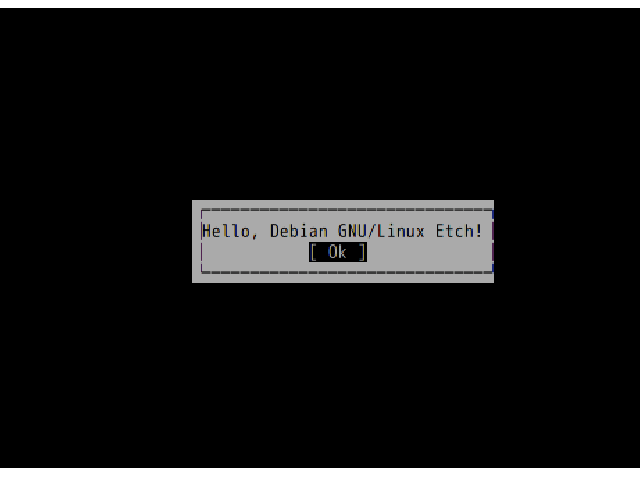
\includegraphics[width=8cm]{image200902/hello-cw.png}
\end{center}

\end{frame}

\begin{frame}[containsverbatim]
ここまではサンプルプログラムの動作確認です。動作しないプログラムをパッケー
ジ化してもしょうがないので、先にどのようなソフトウェアなのか理解するため
にもパッケージング化する前にソースコード等を読んでおくことをお勧めします。
\end{frame}

\emtext{パッケージの雛形}

\begin{frame}[containsverbatim]

{\bf dh\_make}コマンドでパッケージの雛形を作成することができます。
{\bf dh\_make}は、{\bf dh-make}パッケージで提供されています。
以下のコマンドを実行し、インストールします。
\begin{commandline}
$ sudo apt-get install dh-make
\end{commandline}
\end{frame}

\begin{frame}[containsverbatim]

雛形の作成は以下のコマンドを実行します。
\begin{commandline}
$ dh_make --createorig -s
\end{commandline}
{\bf --createorig}オプションはオリジナルソースコードのtar.gzイメージを構築し
  ます。 今回はシングルバイナリパッケージ(一つのソースコードから一つの
  バイナリパッケージが作成される)なので{\bf -s} を指定します。実行すると以下
  のようなメッセージが表示されるので、Enterキーを押します。
\begin{commandline}
Maintainer name : Nobuhiro Iwamatsu
Email-Address   : iwamatsu@nigauri.org 
Date            : Sun, 15 Feb 2009 23:51:58 +0900
Package Name    : hello-cwidget
Version         : 0.1
License         : blank
Using dpatch    : no
Using quilt     : no
Type of Package : Single
Hit <enter> to confirm: 
\end{commandline}
\end{frame}


\begin{frame}[containsverbatim]{debianディレクトリ}
うまく動作すると、{\bf debianディレクトリ}が作成され、この中に雛形が作成され
ます。パッケージメンテナはこのディレクトリの中以外は触りません。
\end{frame}

\begin{frame}[containsverbatim]
\begin{commandline}
.
|-- README.Debian  (Debianパッケージの README)
|-- changelog      (Debianパッケージのチェンジログ)
|-- compat         (Debianパッケージのバージョン)
|-- control        (Debianパッケージ情報)
|-- copyright      (コピーライト情報)
|-- cron.d.ex      (cron を使うパッケージ用設定ファイル)
|-- dirs           (作成するディレクトリ名を指定する)
|-- docs           (インストールするドキュメントファイルを指定する)
|-- emacsen-install.ex (emacs 用設定ファイル)
|-- emacsen-remove.ex  (emacs 用設定ファイル)
|-- emacsen-startup.ex (emacs 用設定ファイル)
|-- hello-cwidget.default.ex (debfonf用)
|-- hello-cwidget.doc-base.EX (doc-base用)
\end{commandline}
\end{frame}

\begin{frame}[containsverbatim]
\begin{commandline}
|-- init.d.ex      (init.dを使うパッケージ用設定ファイル)
|-- init.d.lsb.ex  (init.dを使うパッケージ用設定ファイル)
|-- manpage.1.ex   (manpage の雛形)
|-- manpage.sgml.ex(manpage の雛形)
|-- manpage.xml.ex (manpage の雛形)
|-- menu.ex        (メニューの雛形)
|-- postinst.ex    (postinstメンテナファイルの雛形)
|-- postrm.ex      (postrmメンテナファイルの雛形)
|-- preinst.ex     (preinstメンテナファイルの雛形)
|-- prerm.ex       (prermメンテナファイルの雛形)
|-- rules          (パッケージビルドスクリプト)
`-- watch.ex       (アップストリームチェック用ファイル)
\end{commandline}
\end{frame}

\begin{frame}{CDBS}
./configure ; make ; make install でパッケージのコンパイルができる
ソフトウェアは cdbs を使った方が容易にDebianパッケージ化できます。
\end{frame}


\begin{frame}[containsverbatim]{一回 hello-cwidgetディレクトリを削除する}
現状では先ほどの{\bf dh\_make}の結果が残っているので一回、サンプルプログ
ラムのディレクトリごと削除し、再度展開します。
\begin{commandline}
$ cd 
$ rm -rf hello-cwidget-0.1.*
$ tar -xzf /live/image/osc/data/hello-cwidget-0.1.tar.gz
$ cd hello-cwidget-0.1
\end{commandline}
\end{frame}

\begin{frame}[containsverbatim]{dh\_makeを実行し、パッケージの雛形を作成する}

{\bf CDBS}を使うDebianパッケージの雛形作成は以下のコマンドを実行します。
\begin{commandline}
$ dh_make --createorig -b
\end{commandline}
{\bf -b}オプションを指定すると、CDBS を使った雛形を作成します。
\end{frame}

\begin{frame}[containsverbatim]
\begin{commandline}
Maintainer name : Nobuhiro Iwamatsu
Email-Address   : iwamatsu@nigauri.org 
Date            : Sun, 15 Feb 2009 23:51:58 +0900
Package Name    : hello-cwidget
Version         : 0.1
License         : blank
Using dpatch    : no
Using quilt     : no
Type of Package : cdbs
Hit <enter> to confirm: 
\end{commandline}
\end{frame}

\begin{frame}[containsverbatim]{不要なファイルの削除}
今回のパッケージ化に必要ではないファイルを{\bf debian}ディレクトリ以下から削除
します。
\begin{commandline}
$ rm -rf debian/*.ex debian/*.EX
\end{commandline}
\end{frame}

\begin{frame}[containsverbatim]{debian/changelogファイルの編集}

{\bf debian/changelog}ファイルには{\bf ITP}(Intent To Package)
のバグが既に書かれているで削除します。以下のように変更します。
\begin{commandline}
hello-cwidget (0.1-1) unstable; urgency=low

  * Initial release.

 -- Nobuhiro Iwamatsu <iwamatsu@nigauri.org> \
                  Wed, 18 Feb 2009 16:31:25 +0000

\end{commandline}
\end{frame}

\begin{frame}[containsverbatim]{debian/copyrightファイルの編集}
\begin{commandline}
This package was debianized by Nobuhiro Iwamatsu \ 
                                <iwamatsu@nigauri.org> on
Wed, 18 Feb 2009 16:31:25 +0000.

It was downloaded from <http://www.nigauri.org/~iwamatsu/>

Upstream Author:

    Nobuhiro Iwamatsu <iwamatsu@nigauri.org>

Copyright:

    Copyright (C) 2009 Nobuhiro Iwamatsu <iwamatsu@nigauri.org>

License:

    GPLv2

The Debian packaging is (C) 2009, Nobuhiro Iwamatsu \ 
        <iwamatsu@nigauri.org> and
is licensed under the GPL, see `/usr/share/common-licenses/GPL'.
\end{commandline}
\end{frame}

\begin{frame}[containsverbatim]{debian/controlファイルの編集}
\begin{commandline}
Source: hello-cwidget
Section: devel
Priority: extra
Maintainer: Nobuhiro Iwamatsu <iwamatsu@nigauri.org>
Build-Depends: cdbs, debhelper (>= 7), autotools-dev
Standards-Version: 3.8.0
Homepage: http://www.nigauri.org/~iwamatsu/

Package: hello-cwidget
Architecture: any
Depends: ${shlibs:Depends}, ${misc:Depends}
Description: Debian Packaging Hands-on sample program
 This is sample program of Debian Hands-on done with
 OSC2009 TOKYO Spring.
 This is very easy program that uses CWidget.
\end{commandline}
\end{frame}

\begin{frame}[containsverbatim]{パッケージのビルド}

パッケージのビルドには{\bf debuild}コマンド を使います。
debuildコマンドは{\bf devscripts}パッケージで提供されています。
また、まだ {\bf CDBS}パッケージをインストールしていないので、一緒にイン
ストールします。
パッケージをインストールしたら、パッケージのビルドをしてみましょう。
\begin{commandline}
$ sudo apt-get install devscripts cdbs
$ debuild -us -uc
...
dpkg-buildpackage: full upload (original source is included)
Now running lintian...
W: hello-cwidget: binary-without-manpage usr/bin/hello
W: hello-cwidget: new-package-should-close-itp-bug
Finished running lintian.
\end{commandline}
\end{frame}

\begin{frame}[containsverbatim]{パッケージのインストール}
パッケージが無事ビルドできたら、実際にインストールしてみます。
インストールには dpkg コマンドを使ってインストールします。インストールし
たら、実際に動くか確認してみましょう。
\begin{commandline}
$ sudo dpkg -i ../hello-cwidget_0.1-1_i386.deb
$ which hello
$ hello
\end{commandline}
\end{frame}

\begin{frame}{パッケージのビルドテスト}
パッケージができたあとにはパッケージのテストを行います。
パッケージのビルドテストには{\bf pbuilder}を使います。
pbuilderはDebianに必要な最低限の環境からビルドを行い、
依存関係等のチェックを行ってビルドテストを行うツールです。
\end{frame}

\begin{frame}[containsverbatim]{pbuilderパッケージのインストール}
\begin{commandline}
$ sudo apt-get install pbuilder
\end{commandline}
\end{frame}

\begin{frame}[containsverbatim]{pbuilder環境の構築}

ビルドテストを行う前にbaseシステムイメージを構築する必要があります。
通常は以下のように実行しますが、
\begin{commandline}
$ sudo pbuilder --create --distribution lenny
\end{commandline}
今回はメモリの制限があるため、既に用意してあるbaseシステムイメージを利用
します。イメージは{\bf /live/image/osc/data/base.tgz}にあります。
\end{frame}

\begin{frame}[containsverbatim]{パッケージのビルドテスト}
pbuilder でテストする場合には作成されたパッケージの{\bf dsc}ファイルを指定し
ます。このファイルには、Debianパッケージの構成に必要なファイル名が書かれ
ているので、その情報を元に再ビルドを行うことができます。
また、実行前に{\bf apt-get clean}コマンドを実行してキャッシュをクリアし
てください。メモリが足りないためです。
\begin{commandline}
$ cd ..
$ sudo apt-get clean
$ sudo pbuilder --build --distribution lenny \ 
     --basetgz /live/image/osc/data/base.tgz \
     --buildplace /tmp hello-cwidget_0.1-1.dsc
...
\end{commandline}
\end{frame}

\begin{frame}{なぜエラーになるのか}
先ほどの手順でやってもビルドエラーになります。
なぜエラーになるのでしょうか。考えてみましょう。
\end{frame}

\begin{frame}[containsverbatim]{エラーの原因}
ビルドに必要なパッケージが指定されていないために、この問題は発生します。
正しいhello-cwidgetパッケージの依存関係を見てみます。
\end{frame}

\begin{frame}
\begin{center}
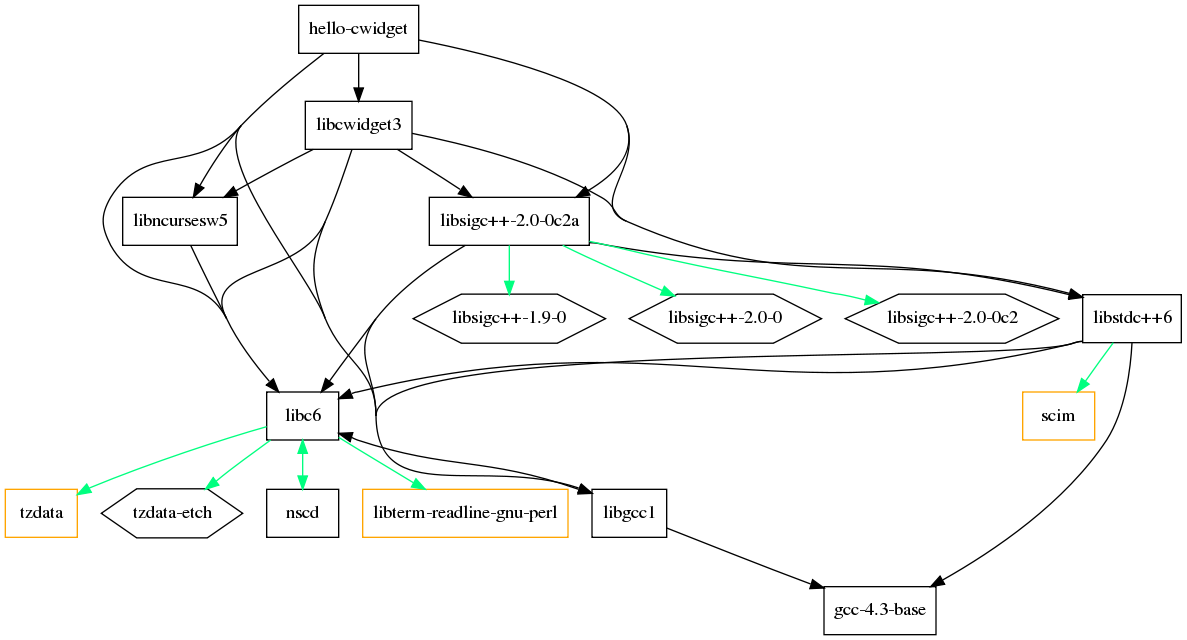
\includegraphics[width=11.5cm]{image200902/cwidget.png}
\end{center}
\end{frame}

\begin{frame}[containsverbatim]
debian/control ファイルを見てみます。

\begin{commandline}
Source: hello-cwidget
Section: devel
Priority: extra
Maintainer: Nobuhiro Iwamatsu <iwamatsu@nigauri.org>
Build-Depends: cdbs, debhelper (>= 7), autotools-dev
Standards-Version: 3.8.0
Homepage: http://www.nigauri.org/~iwamatsu/

Package: hello-cwidget
Architecture: any
Depends: ${shlibs:Depends}, ${misc:Depends}
Description: Debian Packaging Hands-on sample program
 This is sample program of Debian Hands-on done with
 OSC2009 TOKYO Spring.
 This is very easy program that uses CWidget.
\end{commandline}
\end{frame}


\begin{frame}[containsverbatim]{再ビルドテスト}
エラーになる理由は先にインストールしたパッケージ{\bf libcwidget-dev}をパッケー
ジビルド時の依存関係を記述するフィールド{\bf Build-Depends}に追加してい
ないためです。追加して、再ビルドしてみます。

debian/control ファイルを以下のように修正します。

\begin{commandline}
...
Maintainer: Nobuhiro Iwamatsu <iwamatsu@nigauri.org>
Build-Depends: cdbs, debhelper (>= 7), autotools-dev, libcwidget-dev
...
\end{commandline}
\end{frame}

\begin{frame}[containsverbatim]
再ビルドには以下のように実行します。今度はうまくビルドができるはずです。
\begin{commandline}
$ sudo pdebuild -- --distribution lenny --basetgz \
 /live/image/osc/data/base.tgz --buildplace /tmp
\end{commandline}
\end{frame}


\begin{frame}{パッケージのインストール/アンインストールテスト}
パッケージがビルドできただけでは喜んではいけません。インストール/アンイ
ンストールのテストも行いましょう。
パッケージのインストール/アンインストールのテストには{\bf piuparts}パッ
ケージを使います。
\end{frame}

\begin{frame}[containsverbatim]{piupartsのインストール}
以下のように実行し、インストールします。
\begin{commandline}
$ sudo apt-get install piuparts
\end{commandline}
\end{frame}

\begin{frame}[containsverbatim]{パッケージのインストール/アンインストールテスト}
piupartsもpbuilderと同様に最低限の環境からのインストールをチェックします。
よって、baseシステムイメージが必要です。普段は指定する必要はありませんが、
今回は{\bf -b}オプションを付けて、{\bf /live/image/osc/data/base.tgz}に
あるbaseシステムイメージを指定して実行します。
\begin{commandline}
$ cd ..
$ sudo piuparts -d lenny -b /live/image/osc/data/base.tgz \
   hello-cwidget_0.1-1_i386.deb
...
0m41.9s DEBUG: Removed directory tree at /tmp/tmpHliOKO
0m41.9s INFO: PASS: All tests.
0m41.9s INFO: piuparts run ends.
\end{commandline}
\end{frame}

\begin{frame}{プログラムの編集}
hello-cwidgetを実行して、違和感のある方がおられたと思います。
そう、{\bf Lenny}がリリースされたというのに{\bf Etch}になっていました。
これはよくないので変更してみます。今回はよく利用されている{\bf dpatch}
を使って説明します。
\end{frame}

\begin{frame}[containsverbatim]{dpatchのインストール}
dpatchをインストールするには、以下のように実行します。
\begin{commandline}
$ sudo apt-get install dpatch
\end{commandline}
\end{frame}

\begin{frame}[containsverbatim]{dpatchを使うための準備}
dpatchを使う前に、{\bf debian/rules}ファイルにdpatchを使うように設定する必要が
あります。dpatchは一回、パッケージの状態を初期化してから行うためです。
{\bf hello-cwidget-0.1} ディレクトリに移動して、{\bf debian/rules}を以下のように修正します。

\begin{commandline}
$ cd  hello-cwidget-0.1
\end{commandline}

\begin{commandline}
#!/usr/bin/make -f

include /usr/share/cdbs/1/rules/debhelper.mk
include /usr/share/cdbs/1/class/autotools.mk
include /usr/share/cdbs/1/rules/dpatch.mk
include /usr/share/dpatch/dpatch.make
\end{commandline}
\end{frame}


\begin{frame}[containsverbatim]{dpatchの実行}
dpatchは自パッケージを一回コピーし、dpatch環境に移行します。
その中で変更して、dpatch環境を終了する時に差分を作成します。
dpatch環境に移行するには{\bf dpatch-edit-patch}コマンドに
作成する差分を保存するファイル名を指定して実行します。
以下のように実行してください。
\begin{commandline}
$ dpatch-edit-patch 01_change_dist
\end{commandline}
\end{frame}


\begin{frame}[containsverbatim]{ファイルの変更}
今回変更するファイルは{\bf src/hello.cc}です。
エディタを起動し、対象のファイルを変更します。mousepadの場合は以下のよう
に実行します。
\begin{commandline}
$ mousepad ./src/hello.cc
\end{commandline}
{\bf Etch}の部分を{\bf Lenny}に変更したあと、保存してエディタを
終了します。
\end{frame}


\begin{frame}[containsverbatim]{dpatch環境を終了する}
dpatch環境を終了するには以下のように実行してください。
実行すると、差分をファイルに保存してdpatch環境を終了します。
\begin{commandline}
$ exit
\end{commandline}
\end{frame}

\begin{frame}[containsverbatim]{作成された差分(patch)の中身}
作成された差分は\\
{\bf debian/patches/01\_change\_dist.dpatch}
として保存されています。以下のような内容になっているはずです。
\begin{commandline}
#! /bin/sh /usr/share/dpatch/dpatch-run
## 01_change_dist.dpatch by Nobuhiro Iwamatsu <iwamatsu@nigauri.org>
##
## All lines beginning with `## DP:' are a description of the patch.
## DP: No description.

@DPATCH@
diff -urNad hello-cwidget-0.1~/src/hello.cc hello-cwidget-0.1/src/hello.cc
--- hello-cwidget-0.1~/src/hello.cc 2009-02-15 06:56:01.000000000 +0000
+++ hello-cwidget-0.1/src/hello.cc  2009-02-18 16:54:40.668274925 +0000
@@ -26,7 +26,7 @@
    toplevel::init();

    widgets::widget_ref dialog =
-       dialogs::ok(L"Hello, Debian GNU/Linux Etch!",
+       dialogs::ok(L"Hello, Debian GNU/Linux Lenny!",
            util::arg(sigc::ptr_fun(toplevel::exitmain)));

    toplevel::settoplevel(dialog);
\end{commandline}
\end{frame}

\begin{frame}[containsverbatim]
パッチにはなぜそのような説明をしたのか、説明を書く必要があります。
{\bf \#\# DP: No description.}の部分に説明を書きます。
以下のように変更するといいかもしれません。
\begin{commandline}
## DP: Change distributin name from Etch to Lenny.
\end{commandline}
\end{frame}

\begin{frame}[containsverbatim]{作成した差分をパッケージに反映させる}
差分は作成されましたが、このままではパッケージ作成時に差分が適用され
ません。dpatchを使って差分をパッケージに適用させるには{\bf
debian/patches/00list}ファイルを作成し、パッケージに
パッチをファイルに列挙する必要があります。{\bf debian/patches/00list}を
以下のように変更します。
\begin{commandline}
01_change_dist.dpatch
\end{commandline}
\end{frame}

\begin{frame}[containsverbatim]{差分を適用したパッケージを作成する}
差分を適用したパッケージを作成するには通常のパッケージ作成と変わりません。
{\bf debuild}コマンドを使って作成します。
\begin{commandline}
$ debuild -us -uc
....
\end{commandline}
\end{frame}

\begin{frame}{パッケージ作成エラーになる}
説明どおりに操作している人は、パッケージ作成エラーになると思います。
理由は何なのか、考えてみましょう。原因が分かった人は、再ビルドした後に、実際に
インストールして、差分が反映されているか確認してください。
もちろん{\bf pbuilder}/{\bf piuparts}を使ってパッケージのテストを行う事も忘れずに。
\end{frame}

\begin{frame}{質疑応答}
以上で、本ハンズオンは終了です。何か質問等はありますか?
\end{frame}

\begin{frame}{パッケージの問題}
このパッケージにはまだ説明していない2つの問題があります。
\begin{itemize}
\item dpatch による debian/changelog の変更ができていない
\item debian/copyright の copyright が間違っている。
\end{itemize}

\end{frame}

\emtext{次回の勉強会}
\begin{frame}{次回の勉強会}
\begin{itemize}
\item 2008年3月21日は東京大学で開催予定です。
\item 2008年3月7日に関西エリアDebian勉強会が行われます。
\end{itemize}

\end{frame}

\end{document}

;;; Local Variables: ***
;;; outline-regexp: "\\([ 	]*\\\\\\(documentstyle\\|documentclass\\|emtext\\|section\\|begin{frame}\\)\\*?[ 	]*[[{]\\|[]+\\)" ***
;;; End: ***
